%% Wiki: [[2026.01.23 - Mathematics: Spectral Anonymity and Optimal Distinguishing Bounds for Random-Walk Delegation in (Possibly Directed) Overlays]]
\documentclass[11pt]{article}

% -------------------- layout and typography --------------------
\usepackage[margin=1in]{geometry}
\usepackage{microtype}
\setlength{\emergencystretch}{2.5em}

% -------------------- math --------------------
\usepackage{amsmath,amssymb,amsthm,mathtools}

% -------------------- tables and lists --------------------
\usepackage{booktabs}
\usepackage{graphicx}
\usepackage{tabularx}
\usepackage{array}
\usepackage{enumitem}

% -------------------- plots (optional, self-contained) --------------------
\usepackage{pgfplots}
\pgfplotsset{compat=1.18}

% -------------------- hyperlinks and references --------------------
\usepackage[hidelinks]{hyperref}
\usepackage[nameinlink,noabbrev]{cleveref}

% -------------------- theorem environments --------------------
\newtheorem{theorem}{Theorem}[section]
\newtheorem{lemma}[theorem]{Lemma}
\newtheorem{corollary}[theorem]{Corollary}
\newtheorem{definition}[theorem]{Definition}
\newtheorem{proposition}[theorem]{Proposition}
\newtheorem{remark}[theorem]{Remark}

% -------------------- convenient columns --------------------
\newcolumntype{Y}{>{\raggedright\arraybackslash}X}
\newcolumntype{L}[1]{>{\raggedright\arraybackslash}p{#1}}

% -------------------- macros --------------------
\newcommand{\TV}{\mathrm{TV}}
\newcommand{\KL}{\mathrm{KL}}
\newcommand{\E}{\mathbb{E}}
\newcommand{\Prb}{\mathbb{P}}
\newcommand{\defeq}{\stackrel{\mathrm{def}}{=}}
\newcommand{\Unif}{\mathrm{Unif}}
\newcommand{\cD}{\mathcal{D}}
\newcommand{\cM}{\mathcal{M}}
\newcommand{\PiM}{\Pi}

\title{Spectral Anonymity and Optimal Distinguishing Bounds\\for Random-Walk Delegation in (Possibly Directed) Overlays}
\author{}
\date{January 23, 2026}

\begin{document}
\maketitle

\noindent\textbf{Canonical wiki page:} \texttt{[[2026.01.23 - Mathematics: Spectral Anonymity and Optimal Distinguishing Bounds for Random-Walk Delegation in (Possibly Directed) Overlays]]}\\


\begin{abstract}
A common anonymity pattern in overlay routing is \emph{random-walk delegation}:
an initiator performs a short random walk to pick a \emph{delegate} and asks the
delegate to execute a normal lookup. We develop a compact, proof-oriented
anonymity theory for delegate-only observers.

Our organizing lens is structural: under a stationary initiator prior, the
posterior distribution of the initiator given the observed delegate is exactly
the $t$-step law of the \emph{time-reversed} chain started at that delegate.
This reduction turns delegate-only anonymity questions into standard mixing
questions (including on directed/nonreversible overlays). We derive sharp
distinguishing bounds in total variation distance and give leakage certificates:
a conservative $\sigma_2^t$ bound via $\ell_2(\pi)$ contraction and an \emph{exact}
expected $\chi^2$ (R\'enyi-2) leakage identity in terms of the \emph{full}
singular spectrum of the $t$-step discriminant operator $\cD^t$ (which, for
normal/reversible chains, reduces to powers of the one-step spectrum).

For space, this manuscript includes a \emph{reconstruction specification} and a
small set of \emph{sanity-check tables} rather than embedding full logs.
The source-only supplement shipped in this archive at
\texttt{published/2026-01-23\_spectral\_anonymity/supplement/}
contains the reconstruction script and raw sanity anchors, including observation-channel, joint-observation composition, adaptive-transcript composition, post-processing/coarsening, tail-under-coarsening, finite-truncation tail accounting, empirical mixture-law uncertainty, kernel/model uncertainty, numeric/serialization precision, positive-marginal support trimming, hidden-versus-visible selector, adaptive/initiator-correlated selector, prior-scope,
prior-baseline-minimum, prior-composition, visible-hopcount, stochastic-estimator certification, estimator-confidence/multiplicity accounting, pairwise/session support, stop-time-visibility, tail-quantile, separation-vs-upper-ratio, and PML/MaxL guards; rendered plots/logs are left
unshipped as transient artifacts.
\end{abstract}

\section{Introduction}\label{sec:intro}
Many privacy-preserving overlay protocols hide who initiated a lookup by
forwarding the request through one or more intermediate relays, often selected
by random walks. Random-walk selection appears across anonymous DHT lookup and
relay-discovery systems (e.g., Octopus~\cite{octopus}, ShadowWalker~\cite{shadowwalker}, NISAN~\cite{nisan}) and in early
foundational models such as Crowds.

\paragraph{Primitive (fixed-length delegation).}
An initiator $S$ runs a length-$t$ random walk on the overlay to sample a
delegate $D$, then asks $D$ to execute a standard lookup. Our core threat model
assumes the adversary learns only the delegate identity $D$ for a single
delegation. (We briefly discuss ``first-hit'' compromise observations in
\cref{sec:compromise}.)

\paragraph{What is new here.}
The posterior-as-time-reversal identity is elementary, but it is \emph{useful as
a reduction}: it makes the anonymity analysis of delegation \emph{exactly} a
mixing analysis problem, including for directed/nonreversible overlays. The
main technical contributions are the resulting optimal distinguishability bounds
and computable leakage certificates for directed chains, including a
t-step full-spectrum/Frobenius identity (not only a $\sigma_2$ contraction bound).

\paragraph{Main results.}
Let $P$ be the walk kernel on node set $V$ with stationary $\pi$ and let $P^\star$
be its time reversal.
\begin{itemize}[leftmargin=1.2em]
\item \textbf{Posterior structure (tool).} Under $S\sim\pi$, the posterior is a
reversed walk: $\Prb[S=\cdot\mid D=d]=(P^\star)^t(d,\cdot)$ (\cref{thm:posterior}).
\item \textbf{Optimal tests.} Any test distinguishing two candidate initiators
from the delegate identity has optimal advantage equal to total variation
distance between their delegate laws (\cref{cor:opt-test}).
\item \textbf{Spectral certificates, including full spectrum.} Let
$\cD=\Pi^{1/2}P\Pi^{-1/2}$ be the discriminant operator with singular values
$1=\sigma_1\ge\sigma_2\ge\cdots\ge\sigma_n$, and let $\tau_i(t)$ denote the
singular values of $\cD^t$. We give (i) a conservative bound
$\E[\chi^2(\Pr[S=\cdot\mid D]\|\pi)]\le (n-1)\sigma_2^{2t}$ and (ii) an exact identity
$\E[\chi^2(\Pr[S=\cdot\mid D]\|\pi)]=\sum_{i=2}^n\tau_i(t)^2=\|\cD^t\|_F^2-1$
(\cref{thm:chi2-exact}). For normal $\cD$ (in particular, reversible chains) this reduces to $\sum_{i=2}^n\sigma_i^{2t}$.
\item \textbf{Perfect delegation.} Stopping at a strong stationary time yields a
delegate distributed exactly as $\pi$ and independent of $S$ (perfect anonymity
against delegate-only observers; \cref{sec:sst}).
\item \textbf{Non-normal cautionary example.} Directed de Bruijn overlays mix in
finite time yet can have $\sigma_2\approx 1$, making $\sigma_2^t$ bounds vacuous
(\cref{sec:debruijn}).
\end{itemize}

\paragraph{Limitations (explicit).}
This paper deliberately targets \emph{delegate-only} observation, a stationary
initiator prior for the clean spectral certificates, and a \emph{fixed} kernel
$P$, with one exact common-stationary time-inhomogeneous extension recorded in
\cref{prop:inhom,cor:inhom-chi2}.  Non-stationary initiator priors require the
prior-aware identity in \cref{prop:prior-aware} or an evaluator certificate
instead of the stationary-prior shortcut. We do \emph{not} model
global passive traffic analysis (timing/volume correlation, batching, packet
sizes), active/adaptive adversaries (e.g., dropping/biasing forwarding,
Sybil/route-capture), or multi-point observation beyond the delegate identity.
Operational churn outside the common-stationary setting should be read as a
snapshot/perturbation regime: certificates can become stale and degrade toward a
noise floor as churn ``resets'' the mixing clock.

\paragraph{Artifacts and reconstruction.}
To keep the manuscript compact, we include a reconstruction specification and
sanity-check tables in the paper, and ship the source-only reconstruction script
and raw sanity anchors under
\texttt{published/2026-01-23\_spectral\_anonymity/supplement/}.


\section{How to read and verify (LLM-friendly)}\label{sec:howtoread}
This paper is organized around two ``hinge'' facts that let you translate
delegation anonymity questions into standard Markov-chain objects.

\begin{itemize}[leftmargin=1.2em]
\item \textbf{Hinge 1 (posterior as time reversal).} Given a delegate $D=d$ under
a stationary initiator prior, the posterior on the initiator is \emph{exactly}
a reversed walk started at $d$ (\cref{thm:posterior}). You can treat this as a
reduction: any bound on how fast a chain ``forgets its start'' can be imported
as an anonymity statement for delegation.
\item \textbf{Hinge 2 (expected $\chi^2$ leakage as a t-step spectrum).} The expected
R\'enyi-2 leakage has an \emph{exact} formula in terms of the singular spectrum
of the t-step discriminant operator $\cD^t$ (\cref{thm:chi2-exact}). This supplies a computable
certificate that remains informative for directed/non-normal overlays where the
single-number $\sigma_2$ bound can be misleading. Only in the normal/reversible case may one replace the singular values of $\cD^t$ by t-th powers of the one-step singular values.
\end{itemize}

\paragraph{Fast verification path.}
A quick referee-style check is:
(i) verify \cref{thm:posterior} by Bayes + time reversal;
(ii) verify \cref{thm:chi2-exact} by rewriting expected collision probability as a Frobenius norm;
(iii) reproduce \cref{tab:families,tab:firsthit-sweep} from the reconstruction spec in \cref{sec:reconstruct}.
The shipped source-only supplement contains the reconstruction script, raw table anchors, fixed-kernel/schedule self-checks, an observation-channel sanity check, an ergodicity-floor sanity check, hidden-versus-revealed length checks, finite truncation-tail accounting checks, empirical mixture-law uncertainty checks, kernel/model uncertainty checks, numeric/serialization precision checks, positive-support trimming checks, hidden-versus-visible selector checks, adaptive/initiator-correlated selector checks, joint-observation composition checks, adaptive-transcript history-scope checks, success-only/censoring conditioning checks, tail-under-coarsening checks, positive-marginal support trimming checks, arbitrary-prior, prior-baseline-minimum, prior-composition, post-processing/coarsening, stochastic-estimator certification, confidence-accounting, and multiplicity/model-selection checks, separation-vs-upper-ratio checks, pairwise/session support checks, and stop-time visibility checks, and expected-$\chi^2$ to tail/quantile/PML/MaxL translation checks for receipt-side reuse.

\section{Related work and context}\label{sec:related}
Random-walk-based relay selection has a long history in anonymity systems, from
early models such as \emph{Crowds} to anonymous lookup schemes for structured
overlays. Our focus is deliberately narrow: we isolate the \emph{delegation}
primitive and ask what can be inferred from the \emph{delegate identity alone}.
This lens complements system papers that treat richer adversaries (timing,
volume, route-capture, Sybils) by providing sharp and composable bounds for the
delegate-only component.

For concrete systems that instantiate random-walk relay selection and/or anonymous lookup in structured overlays, see ShadowWalker~\cite{shadowwalker} (random-walk-based peer-to-peer anonymity over structured topologies), NISAN~\cite{nisan} (DHT-based network information service for anonymization networks), and Octopus~\cite{octopus} (secure and anonymous DHT lookup).

On the Markov-chain side, we use standard notions from mixing theory---total
variation and separation distance, time reversal, and strong stationary times.
Background can be found in Levin--Peres--Wilmer \cite{lpw} and in the original
strong-stationary-time work of Aldous--Diaconis \cite{aldousdiaconis}; see also
Fill \cite{fill} for related perspectives. On the systems side, our results
provide a principled way to interpret (and sometimes refute) common heuristics
that ``a spectral gap guarantees privacy,'' especially for directed overlays.
We also relate to work on adding query privacy to robust DHTs \cite{backes} and
to classic relay-anonymity models \cite{reiterrubin}.

\section{Model and definitions}\label{sec:model}
Let $V$ be a finite set of nodes, $|V|=n$. Let $P$ be a (row-stochastic) Markov
kernel on $V$ with stationary distribution $\pi$ satisfying $\pi(x)>0$ for all
$x$. We allow $P$ to be directed and nonreversible.

\paragraph{Delegation experiment.}
Sample an initiator $S\sim \pi$. Starting from $S$, run the chain for $t$ steps
and output the endpoint $D$ (the delegate):
\[
\Prb[D=d\mid S=s] = P^t(s,d).
\]

\paragraph{Time reversal.}
Define the time-reversed kernel $P^\star$ by
\begin{equation}\label{eq:rev}
\pi(x)P(x,y)=\pi(y)P^\star(y,x)\qquad(\forall x,y\in V),
\end{equation}
so $P^\star(y,x)=\pi(x)P(x,y)/\pi(y)$.

\paragraph{Distances and leakage.}
For distributions $\mu,\nu$ on $V$,
\[
\TV(\mu,\nu)=\tfrac12\sum_{x\in V}|\mu(x)-\nu(x)|.
\]
The Pearson chi-squared divergence is
\[
\chi^2(\mu\|\pi)=\sum_{x\in V}\frac{(\mu(x)-\pi(x))^2}{\pi(x)}
=\sum_{x\in V}\frac{\mu(x)^2}{\pi(x)}-1.
\]
We use conditional min-entropy
$H_\infty(S\mid D)= -\log \sum_d \Prb[D=d]\max_s \Prb[S=s\mid D=d]$.

\section{Posterior structure and optimal tests}\label{sec:posterior}
\begin{theorem}[Posterior equals reversed walk]\label{thm:posterior}
Assume $S\sim \pi$ and $D$ is obtained by a length-$t$ walk from $S$ using $P$.
Then for every $d\in V$,
\[
\Prb[S=s\mid D=d] = (P^\star)^t(d,s)\qquad(\forall s\in V).
\]
\end{theorem}
\begin{proof}
Bayes' rule gives
$\Prb[S=s\mid D=d]=\frac{P^t(s,d)\pi(s)}{\sum_u P^t(u,d)\pi(u)}$.
Stationarity implies $\sum_u \pi(u)P^t(u,d)=\pi(d)$, hence
$\Prb[S=s\mid D=d]=\pi(s)P^t(s,d)/\pi(d)$. Applying \eqref{eq:rev} $t$ times
yields $\pi(s)P^t(s,d)=\pi(d)(P^\star)^t(d,s)$.
\end{proof}

\begin{proposition}[Arbitrary-prior observation-channel identity]\label{prop:prior-aware}
Let an observation channel from initiators to a finite observation alphabet be
$W(s,y)=\Prb[Y=y\mid S=s]$. Let the initiator prior be a full-support distribution
$\rho$ and write $m(y)=\sum_s\rho(s)W(s,y)$ for the observation marginal.
Let $Y_+=\{y:m(y)>0\}$, let $W_+$ be $W$ restricted to columns in $Y_+$, and
let $m_+$ be the corresponding positive marginal vector.  Zero-marginal
observation columns may be deleted before any inverse square root is formed.  On
the support where $m(y)>0$,
\[
\Prb[S=s\mid Y=y]=\frac{\rho(s)W(s,y)}{m(y)},
\]
and the prior-relative expected $\chi^2$ leakage is
\[
\E_{Y\sim m}\!\left[\chi^2(\Prb[S=\cdot\mid Y]\|\rho)\right]
=\left\|\mathrm{diag}(\sqrt{\rho})W_+\mathrm{diag}(m_+^{-1/2})\right\|_F^2-1.
\]
Taking $W=P^t$ gives the arbitrary-prior delegate formula.  When $\rho=\pi$ and
$W=P^t$, this reduces to \cref{thm:chi2-exact}; when $W=P_1\cdots P_t$ or
$W=\sum_t p_tP^t$, it gives the corresponding schedule or hidden-hopcount
witness.  Thus the exact object is scoped to the declared observation channel,
not just to a kernel name.
\end{proposition}
\begin{proof}
Bayes' rule gives the posterior formula.  Substituting it into the definition of
expected $\chi^2$ gives
\[
\sum_y m(y)\sum_s \frac{\rho(s)^2W(s,y)^2}{m(y)^2\rho(s)}-1
=\sum_{s,y}\frac{\rho(s)W(s,y)^2}{m(y)}-1,
\]
which is exactly the displayed Frobenius norm minus one after restricting to the
positive-marginal support.
\end{proof}

\begin{remark}[Observation-channel support trimming]\label{rem:support-trim}
The display in \cref{prop:prior-aware} is evaluated only on the
positive-marginal observation support.  Equivalently, write $m_+$ for the vector
of positive entries of $m$ and $W_+$ for the corresponding columns of $W$, then
use $\mathrm{diag}(m_+^{-1/2})$.  A zero-marginal observation column has no
posterior event under the declared prior and must be trimmed rather than silently
inverted.  The supplement's \texttt{--support-sanity} check records that adding
or deleting such zero-marginal columns does not change the expected $\chi^2$
value, while making the support convention explicit for receipts.
\end{remark}


\begin{proposition}[Observation coarsening / post-processing monotonicity]\label{prop:postprocess}
Work in the setting of \cref{prop:prior-aware}.  Let $R(y,z)$ be any
row-stochastic post-processing channel from the original observation $Y$ to a
coarsened observation $Z$, independent of $S$ given $Y$, and write
$W_R(s,z)=\sum_y W(s,y)R(y,z)$.  Then
\[
\E_Z\!\left[\chi^2(\Prb[S=\cdot\mid Z]\|\rho)\right]
\le
\E_Y\!\left[\chi^2(\Prb[S=\cdot\mid Y]\|\rho)\right].
\]
Consequently, a certificate for a richer observation can upper-bound any declared
coarsened observation obtained by a certified postprocessor, but not conversely:
a delegate-only or hidden-hopcount certificate cannot be reused for a visible
hopcount / richer transcript observer without recomputing the larger channel.
\end{proposition}
\begin{proof}
For each $z$ with positive marginal $m_Z(z)$,
\[
\Prb[S=\cdot\mid Z=z]
=\sum_{y:m(y)>0}\frac{m(y)R(y,z)}{m_Z(z)}\,\Prb[S=\cdot\mid Y=y].
\]
The weights form a probability distribution.  Since
$\mu\mapsto\chi^2(\mu\|\rho)$ is convex in $\mu$, Jensen's inequality gives the
pointwise bound after conditioning on $Z=z$; averaging over $z$ and using
$\sum_z m_Z(z)\,m(y)R(y,z)/m_Z(z)=m(y)$ proves the claim.
\end{proof}

\begin{remark}[Tail endpoints under coarsening]\label{rem:tail-coarsening}
\Cref{prop:postprocess} is an expectation/data-processing statement.  A
pointwise $\chi^2$ cap transfers through post-processing, and a Markov tail cap
formed from the richer expected leakage remains safe because the coarsened
expectation is no larger.  By contrast, a high-probability tail/quantile endpoint, exact quantile, or
Cantelli-style moment certificate is an event statement over the source
observation alphabet: a small bad rich-observation cell can be merged with many
good cells and turn into a large coarsened cell.  Therefore a rich-channel
quantile or high-probability tail/quantile PML endpoint is not automatically a target-scope quantile after coarsening and must not be copied unchanged.  Receipt
reuse must either recompute the tail bound on the target channel or carry a
coarsening-contamination certificate bounding the target mass touched by source
bad cells.  The supplement's \texttt{--tail-postprocess-sanity} check records a
finite example of this failure mode.
\end{remark}



\begin{proposition}[Joint observations compose as a new channel]\label{prop:joint-observation}
Work in the setting of \cref{prop:prior-aware}.  If two observations $Y$ and
$Z$ are both visible and are conditionally independent given the initiator, with
channels $W_1(s,y)$ and $W_2(s,z)$, then the observer's channel is
\[
W_{\mathrm{joint}}(s,(y,z))=W_1(s,y)W_2(s,z),
\]
and \cref{prop:prior-aware} applies to $W_{\mathrm{joint}}$ after trimming its
positive-marginal support.  More generally, any side channel, transcript field,
or telemetry feature that is not a post-processing of an already-certified
observation must be included in the declared observation channel or bounded by a
separate evaluator composition certificate.
\end{proposition}
\begin{proof}
Conditional independence gives the displayed channel and row stochasticity follows
from the row stochasticity of $W_1$ and $W_2$.  The expected posterior $\chi^2$
identity is then exactly \cref{prop:prior-aware} applied to this enlarged finite
observation alphabet.
\end{proof}

\begin{remark}[Joint-observation receipt guard]
A certificate for one component observation is not a certificate for the jointly
visible transcript.  Joint visibility is not the maximum of individual certificates
and is not a post-processing of either component alone.  A receipt that combines
an endpoint delegate with visible hopcount, selector identity, retry metadata,
traffic class, or another initiator-dependent side channel must either materialize
the joint observation channel, cite a product/full observation-channel evaluator
bound, or fail closed to an estimate-only / not-yet-certified status.
The supplement's \texttt{--joint-observation-sanity} check gives a two-channel
example where each individual expected-$\chi^2$ value is smaller than the joint
value.
\end{remark}

\begin{proposition}[Adaptive transcripts are one observation channel]\label{prop:adaptive-transcript}
Let a finite transcript $H_k=(Y_1,\ldots,Y_k)$ be generated sequentially.  After a
history $h_{j-1}=(y_1,\ldots,y_{j-1})$, the protocol/evaluator uses the actual
history-conditioned channel
\[
  W_j^{h_{j-1}}(s,y_j)=\Prb[Y_j=y_j\mid S=s,H_{j-1}=h_{j-1}].
\]
Then the transcript itself has the observation channel
\[
  W_{\mathrm{tr}}(s,h_k)=\prod_{j=1}^k W_j^{h_{j-1}}(s,y_j),
\]
with zero-probability histories trimmed as in \cref{rem:support-trim}, and
\cref{prop:prior-aware} applies to $W_{\mathrm{tr}}$.  Consequently, a marginal
or initial-prior per-round witness is not automatically a certificate for a
history-visible or policy-adaptive transcript.  Safe reuse needs the full
transcript channel, or a separate adaptive-composition certificate that is
uniform over the declared histories, conditioned priors, support policy, endpoint
kind, and failure-budget allocation.
\end{proposition}
\begin{proof}
The displayed product is just the chain rule for the conditional law of the
finite transcript given the initiator.  Once this product channel is formed, the
posterior-$\chi^2$ identity is exactly \cref{prop:prior-aware}; histories with
zero marginal mass are outside the observation support and are deleted before any
inverse marginal is formed.
\end{proof}

\begin{remark}[Marginal round checks are not transcript checks]\label{rem:adaptive-transcript}
A multi-round receipt can look safe if each field is checked only as a marginal
under the initial prior while the jointly visible transcript reveals the start.
The supplement's \texttt{--adaptive-transcript-sanity} check gives a two-round
binary example: $Y_1$ is an independent fair bit and $Y_2=S\oplus Y_1$.  Both
marginals have zero expected posterior $\chi^2$ under the initial prior, but the
transcript $(Y_1,Y_2)$ reveals $S$ exactly.  Thus receipt cards should record
\texttt{transcript\_scope} and, when they do not materialize the transcript
channel directly, an \texttt{adaptive\_composition} certificate with
history-conditioned priors and endpoint/failure-budget semantics.  Marginal
per-round or delegate-only witnesses fail closed for adaptive/history-visible
transcripts.
\end{remark}

\begin{remark}[Censoring and success-only conditioning]\label{rem:censoring}
A success-only log, abort-filtered transcript, retry-censored trace, or route that emits a receipt only when a hidden event $C$ occurs is not automatically certified by the unconditional delegate witness.  The success/abort status is itself an observation channel; if the status is hidden and only $C$-conditioned traces are analyzed, the reference prior changes to
\[
  \rho\mid C(s)=\frac{\rho(s)\Pr[C\mid S=s]}{\sum_{s'}\rho(s')\Pr[C\mid S=s']},
\]
and the conditional observation channel is $W_C(s,y)=W(s,y)/\Pr[C\mid S=s]$ for $y\in C$.  Thus receipt cards should record \texttt{conditioning\_scope} and \texttt{censoring\_policy}: either include the status as part of the observation channel, or recompute the conditional channel and the conditioned reference prior, including the corresponding \texttt{prior\_min}/\texttt{reference\_min}.  If some start has zero probability of $C$, the conditioned scope loses support and must be treated as a restricted-prior or fail-closed certificate rather than as an unconditional anonymity claim.  The supplement's \texttt{--censoring-sanity} check gives a two-state example where the success-only channel has zero leakage only after the prior is changed, while the success event itself carries the omitted leakage.
\end{remark}

\begin{remark}[Stationary-prior guard]
The spectral identities in \cref{sec:spectral} are the clean stationary-prior
specialization for a delegate-only observation channel.  A receipt or design note
that changes the initiator prior or enlarges the observation (for example from
$D$ to $(D,T)$) must carry the declared prior and observation scope, trim any
zero-marginal observation columns before applying the Frobenius identity, and either
use \cref{prop:prior-aware} directly or rely on a separate evaluator-certified
bound; it should fail closed rather than reusing a stationary $\pi$, hidden-hopcount, hidden-selector,
or delegate-only witness by analogy.  The same fail-closed rule applies when a
selector, stop rule, retry branch, or schedule branch is path-dependent, state-dependent,
or otherwise correlated with the initiator: the unconditional independent-selector
mixture is then not the observation channel and the full induced channel must be
materialized or evaluator-certified.  If the later observation is only coarser,
\cref{prop:postprocess} allows reuse from the richer witness only after the
post-processing / coarsening map is declared, and tail/quantile reuse follows \cref{rem:tail-coarsening}.
\end{remark}

\begin{proposition}[Time-varying kernels]\label{prop:inhom}
The posterior-as-reversal lens extends verbatim to time-inhomogeneous walks.
Let $P_1,\dots,P_t$ be a sequence of Markov kernels that share a stationary
distribution $\pi$ (i.e., $\pi P_i=\pi$ for all $i$). Sample $S\sim\pi$ and run
the inhomogeneous chain $X_0=S$, $X_{i}=X_{i-1}P_i$, and output $D=X_t$.
Then, for every $d\in V$,
\[
\Prb[S=s\mid D=d] \;=\; (P_t^\star P_{t-1}^\star\cdots P_1^\star)(d,s),
\]
where $P_i^\star$ is the time reversal of $P_i$ with respect to $\pi$.
\end{proposition}

\begin{proof}
By Bayes' rule,
$\Prb[S=s\mid D=d]=\pi(s)(P_1\cdots P_t)(s,d)/\pi(d)$, using $\Prb[D=d]=\pi(d)$.
Applying the single-step reversal identity $\pi(x)P_i(x,y)=\pi(y)P_i^\star(y,x)$
along the product yields $(P_t^\star\cdots P_1^\star)(d,s)$.
\end{proof}

\begin{corollary}[Shared-stationary schedule chi-squared witness]\label{cor:inhom-chi2}
Under the hypotheses of \cref{prop:inhom}, define
\[
\cD_i=\PiM^{1/2}P_i\PiM^{-1/2},\qquad
\cM_t=\cD_1\cD_2\cdots\cD_t
=\PiM^{1/2}(P_1P_2\cdots P_t)\PiM^{-1/2}.
\]
If $\eta_i(t)$ are the singular values of the ordered product $\cM_t$, then
\[
\E_{D\sim\pi}\!\left[\chi^2(\Prb[S=\cdot\mid D]\|\pi)\right]
=\|\cM_t\|_F^2-1
=\sum_{i=2}^n\eta_i(t)^2.
\]
If $\sigma_{2,i}$ upper-bounds the restriction of $\cD_i$ to the
stationary-orthogonal subspace, then also
\[
\E[\chi^2]\le (n-1)\prod_{i=1}^t\sigma_{2,i}^{2}.
\]
Thus a time-varying witness must certify the actual ordered product for exact
expected leakage. Products or powers of one-step singular values are conservative
certificates unless an additional normal/commuting/evaluator certificate proves
that a shortcut is exact. As in the fixed-kernel theorem, a receipt-side MaxL
claim must record the tail/pointwise conversion used before treating this
expected value as a \texttt{chi2\_bound}.
\end{corollary}

\begin{proof}
Repeat the proof of \cref{thm:chi2-exact} with
$P^t$ replaced by the product $K=P_1\cdots P_t$. The common-stationary
assumption gives $\pi K=\pi$, and the discriminant of $K$ is exactly the ordered
product $\cM_t$. The stationary singular direction again contributes one unit.
For the conservative bound, restrict each $\cD_i$ to $u^\perp$, where
$u=\sqrt\pi$, and use $\|B_1\cdots B_t\|_F^2\le
(n-1)\prod_i\|B_i\|_2^2$.
\end{proof}

\begin{remark}[Churn as perturbation]
If churn changes the kernel over time while preserving a common stationary
distribution exactly, \cref{prop:inhom,cor:inhom-chi2} give the exact reversal and
ordered-product Frobenius witness for the actual time-varying walk. If the
common-stationary condition only holds approximately, or if stationarity itself
drifts, the snapshot results in this paper should be interpreted as local
guarantees that can degrade toward a noise floor.  The same floor interpretation
applies to reducible or periodic kernels: the Frobenius identity remains exact,
but the non-stationary terms need not decay to zero.
\end{remark}



\begin{remark}[Framing]\label{rem:lens}
\cref{thm:posterior} is a one-line calculation, but it is the key \emph{lens} of
this paper: it converts delegate-only anonymity analysis into standard mixing
analysis on the reversed chain, including for directed/nonreversible overlays.
\end{remark}

\begin{corollary}[Optimal test]\label{cor:opt-test}
For any two candidates $s_0,s_1\in V$ and any (possibly randomized) test
$\phi:V\to\{0,1\}$ based only on $D$,
\[
\max_{\phi}\Big|\Prb[\phi(D)=1\mid S=s_0]-\Prb[\phi(D)=1\mid S=s_1]\Big|
= \TV\!\big(P^t(s_0,\cdot),\,P^t(s_1,\cdot)\big).
\]
\end{corollary}
\begin{proof}
Classical characterization of total variation distance as optimal distinguishing
advantage between two distributions.
\end{proof}

\section{Spectral anonymity bounds}\label{sec:spectral}
For reversible chains, mixing is governed by eigenvalues; for directed chains,
singular values of the \emph{discriminant} operator play the analogous role.

\paragraph{Ergodicity convention and leakage floors.}
The exact Frobenius identities below require only a finite kernel with positive
stationary distribution.  Statements that the non-stationary leakage terms decay
as $t$ grows use the usual finite-chain ergodicity condition
$P^t\to \mathbf{1}\pi$ (for example, irreducible and aperiodic).  If the chain
is reducible or periodic, the same identities still hold, but additional
non-decaying modes remain inside $\sum_{i\ge2}\tau_i(t)^2$ and appear as an
expected-$\chi^2$ leakage floor.  This decay condition should not be confused
with a one-step claim $\sigma_2(\cD)<1$: non-normal ergodic chains can have
$\sigma_2(\cD)=1$ while the actual t-step operator $\cD^t$ still collapses.

\begin{definition}[Discriminant operator]\label{def:disc}
Let $\PiM=\mathrm{diag}(\pi)$. Define
\[
\cD \;=\; \PiM^{1/2} P \PiM^{-1/2}.
\]
Let $1=\sigma_1\ge\sigma_2\ge\cdots\ge\sigma_n\ge 0$ be its singular values.
\end{definition}

\begin{theorem}[Exact expected chi-squared leakage]\label{thm:chi2-exact}
Under the stationary prior, let $\mu_d(\cdot)=\Prb[S=\cdot\mid D=d]$.  Let
$1=\tau_1(t)\ge\tau_2(t)\ge\cdots\ge\tau_n(t)\ge 0$ be the singular values of
$\cD^t$. Then
\[
\E_{D\sim \pi}\!\left[\chi^2(\mu_D\|\pi)\right] \;=\;
\|\cD^t\|_F^2-1
\;=\;
\sum_{i=2}^n \tau_i(t)^2.
\]
If $\cD$ is normal (in particular, if $P$ is reversible), then
$\tau_i(t)=\sigma_i^t$ and the identity reduces to
$\sum_{i=2}^n\sigma_i^{2t}$.
\end{theorem}
\begin{proof}
Let $M=\PiM^{1/2}P^t\PiM^{-1/2}=\cD^t$.  From Bayes' rule and stationarity,
$\mu_d(s)=\pi(s)P^t(s,d)/\pi(d)$.  Hence
\[
\begin{aligned}
\E_{D\sim\pi}\!\left[1+\chi^2(\mu_D\|\pi)\right]
&=\sum_d\pi(d)\sum_s\frac{\mu_d(s)^2}{\pi(s)} \\
&=\sum_{s,d}\frac{\pi(s)P^t(s,d)^2}{\pi(d)} \\
&=\|\PiM^{1/2}P^t\PiM^{-1/2}\|_F^2
=\|\cD^t\|_F^2.
\end{aligned}
\]
The vector $u=\sqrt{\pi}$ is a unit left and right singular vector of
$\cD^t$ with singular value one.  Subtracting this one stationary contribution
therefore gives $\|\cD^t\|_F^2-1=\sum_{i=2}^n\tau_i(t)^2$.  Under ergodicity the
remaining terms decay to zero as $t$ grows; without ergodicity they may include
unit or non-decaying modes, and those modes are exactly the leakage floor rather
than a failure of the identity.  The final specialization follows only when
powers preserve the singular basis, e.g. for normal $\cD$; no such step is used
for directed/non-normal chains.  This theorem is an expectation over $D\sim\pi$;
receipt-side PML, channel-level MaxL, or pointwise posterior statements must
first convert the expected $\chi^2$ value into a tail/pointwise bound (for
example by Markov's inequality, Cantelli's inequality when the variance over
delegates is available, or by an evaluator-certified quantile).
\end{proof}

\begin{remark}[Tail envelopes, PML, and channel-level MaxL]
Let $X_d=\chi^2(\mu_d\|\pi)$, $\pi_{\min}=\min_s\pi(s)$, and
$\ell(d)=\log_2\max_s\mu_d(s)/\pi(s)$ be the realized odds-inflation / PML at
delegate $d$.  A tail certificate $\Pr[X_D\le B]\ge 1-\delta$ gives the
high-probability envelope
\[
\ell(D)\le b_{\mathrm{PML}}(B)\defeq\log_2\min\left\{1+\sqrt{B/\pi_{\min}},\,1/\pi_{\min}
\right\}
\]
with probability at least $1-\delta$.  This is not by itself a channel-level
MaxL budget unless $\delta=0$ or the failure mass is accounted for.  Using the
endpoint-bridge identity $\mathrm{MaxL}=\log_2\E[2^{\ell(D)}]$ and the universal
fallback $2^{\ell(D)}\le 1/\pi_{\min}$ gives the conservative conversion
\[
\mathrm{MaxL}\le\log_2\left((1-\delta)2^{b_{\mathrm{PML}}(B)}+\delta/\pi_{\min}
\right).
\]
Thus Markov, Cantelli, and evaluator-quantile conversions produce
high-probability PML envelopes first; a receipt that advertises channel-level
MaxL must either use a pointwise cap or include this failure-mass fallback.
For the arbitrary-prior observation-channel identity in \cref{prop:prior-aware},
replace $\pi$ throughout this paragraph by the declared reference prior $\rho$
and replace $\pi_{\min}$ by $\rho_{\min}=\min_s\rho(s)$.  A class-prior or
non-stationary-prior receipt must serialize this baseline minimum explicitly;
borrowing an unrelated stationary $\pi_{\min}$ can understate posterior odds and
therefore is not a valid PML/MaxL conversion.
\end{remark}

\begin{corollary}[Conservative $\sigma_2$ certificate]\label{cor:sigma2}
Under the hypotheses of \cref{thm:chi2-exact},
\[
\E_{D\sim\pi}\!\left[\chi^2(\mu_D\|\pi)\right]\le (n-1)\sigma_2^{2t},
\qquad
\E[\TV(\mu_D,\pi)] \le \tfrac12\sqrt{(n-1)}\,\sigma_2^{t}.
\]
\end{corollary}
\begin{proof}
Let $u=\sqrt{\pi}$.  Since $\cD u=u$ and $\cD^\top u=u$, the orthogonal complement
$u^\perp$ is invariant for both $\cD$ and $\cD^\top$.  Write $B$ for the restriction
of $\cD$ to $u^\perp$.  The exact identity above gives
$\E[\chi^2(\mu_D\|\pi)]=\|B^t\|_F^2$.  Therefore
$\|B^t\|_F^2\le (n-1)\|B^t\|_2^2\le (n-1)\|B\|_2^{2t}=(n-1)\sigma_2^{2t}$.
When $\sigma_2=1$ this remains a correct but potentially vacuous certificate;
fast non-normal mixing is why the direct t-step witness is useful.  The TV bound
follows from $\TV(\mu,\pi)\le \frac12\sqrt{\chi^2(\mu\|\pi)}$ and Jensen.
\end{proof}

\paragraph{Why the t-step spectrum matters.}
For non-normal directed chains, $\sigma_2$ can be close to 1 even when the chain
mixes quickly (see \cref{sec:debruijn}); \cref{thm:chi2-exact} can remain sharp
because the singular values of $\cD^t$ may be much smaller than t-th powers of the
one-step singular values.  Do not replace $\tau_i(t)$ by $\sigma_i^t$ unless the
normal/reversible hypothesis is present.

\section{Perfect delegation via strong stationary times}\label{sec:sst}
\begin{definition}[Strong stationary time]
For a chain started from a fixed state $x$, a stopping time $T$ is a
\emph{strong stationary time} if
\[
\Prb_x[X_T=y,\ T=k]=\pi(y)\Prb_x[T=k]\qquad(\forall y,k).
\]
Equivalently, under that fixed start, $X_T\sim\pi$ and $X_T$ is independent of
$T$.  We call a stopping rule \emph{uniformly strong} when this property holds
for every starting state.
\end{definition}

\begin{theorem}[Perfect delegate-only anonymity]
If delegation outputs $D=X_T$ for a uniformly strong stationary time $T$, then
for every start $s$, $\Prb[D=d\mid S=s]=\pi(d)$.  Hence $D$ is independent
of $S$ under any initiator prior, and a delegate-only observer sees the prior
unchanged: $\Prb[S=s\mid D=d]=\Prb[S=s]$.
\end{theorem}
\begin{proof}
The uniformly strong property gives $X_T\sim\pi$ for each fixed start.  Since
the conditional delegate law does not depend on the start, mixing over any prior
on $S$ preserves independence of $D$ and $S$.
\end{proof}

\begin{remark}[Stop-time visibility guard]
The theorem is deliberately delegate-only.  A strong stationary time does not by
itself imply that the pair $(D,T)$ is independent of $S$: the distribution of the
stopping time can depend on the start even while $X_T$ is stationary under each
fixed start.  Thus $T$ itself may leak the initiator if hopcount, latency, or
termination behavior is visible.  Systems that reveal the stopping time need an
additional start-independent stopping-time, halting-state, padding, or evaluator
certificate before claiming perfect anonymity for the enlarged observation.
\end{remark}

\section{Repeated lookups: tensorization}\label{sec:repeated}
Suppose the same initiator performs $k$ independent delegations, producing
delegates $D_1,\dots,D_k$.

\begin{proposition}[Posterior tensorizes]\label{prop:tensor}
Under a stationary prior and conditional independence of walks,
\[
\Prb[S=s\mid D_1=d_1,\dots,D_k=d_k]
\;\propto\; \pi(s)\prod_{j=1}^k P^t(s,d_j).
\]
\end{proposition}
\begin{proof}
Bayes' rule and conditional independence:
$\Prb[D_1=d_1,\dots,D_k=d_k\mid S=s]=\prod_j P^t(s,d_j)$.
\end{proof}

\paragraph{Amplification (interpretation).}
The optimal distinguishing advantage between two candidates from the vector
$(D_1,\dots,D_k)$ is the total variation distance between the corresponding
product laws.  Let $q_s=P^t(s,\cdot)$.  When the needed absolute continuity
condition holds (otherwise the KL/$\chi^2$ bound is infinite and therefore
vacuous), additivity of KL divergence and Pinsker's inequality give the explicit
bound
\[
\KL(q_{s_0}^{\otimes k}\|q_{s_1}^{\otimes k})
  = k\,\KL(q_{s_0}\|q_{s_1}),
\qquad
\TV(q_{s_0}^{\otimes k},q_{s_1}^{\otimes k})
  \le \sqrt{\frac{k\,\KL(q_{s_0}\|q_{s_1})}{2}}
  \le \sqrt{\frac{k\,\chi^2(q_{s_0}\|q_{s_1})}{2}} .
\]
Thus a pairwise single-delegation KL or $\chi^2$ certificate scales linearly in
divergence and as $\sqrt{k}$ in this TV upper bound.  The average posterior
$\chi^2$ certificate in \cref{thm:chi2-exact} should not be reused as this
pairwise law bound unless an evaluator separately certifies that implication for
the candidate pair and prior scope being claimed.

\begin{remark}[Pairwise/session support guard]
Pairwise and session-level endpoints are support-sensitive.  A rare-marker
channel can have small prior-averaged posterior $\chi^2$ while one candidate law
assigns positive probability to an observation that another candidate law forbids,
so the corresponding pairwise KL is infinite and linked repetitions drive TV
quickly toward one.  Consequently a receipt that claims pairwise TV, pairwise KL,
or a linked-session bound must carry pairwise laws, support / absolute-continuity
evidence, and the linkage model; it is not licensed by the average posterior
$\chi^2$ identity alone.  The supplement's
\texttt{--pairwise-session-sanity} check records a finite support mismatch in
which the average posterior leakage is below $0.02$ but 100 linked repetitions
have TV above $0.5$.
\end{remark}


\section{Randomized walk length and hopcount leakage}\label{sec:randlen}
Some systems randomize the walk length (hopcount) to reduce latency or to
complicate inference. Let $T$ be an integer-valued random walk length, sampled
independently of the initiator and of the walk transitions, and let the delegate
be $D=X_T$.

\begin{proposition}[Posterior under randomized length]\label{prop:randlen}
Assume $S\sim\pi$ and $T\perp S$. Then:
\begin{enumerate}[leftmargin=1.6em]
\item If the adversary observes both $(D,T)=(d,t)$, then
$\Prb[S=\cdot\mid D=d,T=t]=(P^\star)^t(d,\cdot)$.
\item If the adversary observes only $D=d$, then the posterior is a mixture of
reversed walks:
\[
\Prb[S=s\mid D=d] \;=\; \sum_{t\ge 0} \Prb[T=t]\,(P^\star)^t(d,s).
\]
\end{enumerate}
\end{proposition}

\begin{proof}
For (1), condition on $T=t$ and apply \cref{thm:posterior}. For (2),
$\Prb[S=s\mid D=d]\propto \pi(s)\sum_t \Prb[T=t]P^t(s,d)$ and the denominator
equals $\pi(d)$ by stationarity; rewrite each term using time reversal.
\end{proof}

\begin{proposition}[Visible versus hidden randomized-length chi-squared leakage]\label{prop:randlen-chi2}
Let $p_t=\Prb[T=t]$.  If the adversary observes both $D$ and $T$, then
\[
\E_{(D,T)}\!\left[\chi^2(\Prb[S=\cdot\mid D,T]\|\pi)\right]
=\sum_{t\ge0}p_t\bigl(\|\cD^t\|_F^2-1\bigr).
\]
If the adversary observes $D$ but not $T$, define the hidden-length mixture
discriminant
\[
M_T=\sum_{t\ge0}p_t\cD^t,
\]
with the obvious finite-dimensional limit for countably supported $T$.  Then
\[
\E_{D\sim\pi}\!\left[\chi^2(\Prb[S=\cdot\mid D]\|\pi)\right]
=\|M_T\|_F^2-1.
\]
Moreover,
\[
\|M_T\|_F^2-1
\le \sum_{t\ge0}p_t\bigl(\|\cD^t\|_F^2-1\bigr),
\]
so hiding a randomized length never increases expected $\chi^2$ leakage relative
to revealing the length and averaging over $T$.
\end{proposition}

\begin{proof}
For the visible-hopcount observation channel, the observation alphabet is pairs
$(t,d)$ and $W(s,(t,d))=p_tP^t(s,d)$.  Under stationarity its marginal is
$p_t\pi(d)$, so \cref{prop:prior-aware} decomposes the expected leakage into the
weighted average of the fixed-length Frobenius identities.  For hidden hopcount,
the delegate kernel is $K_T=\sum_t p_tP^t$, which is stochastic and stationary for
$\pi$.  Its discriminant is $\PiM^{1/2}K_T\PiM^{-1/2}=M_T$, so the Frobenius
identity applies with $P^t$ replaced by $K_T$.  The inequality is convexity of the
squared Frobenius norm:
$\|\sum_t p_t\cD^t\|_F^2\le\sum_t p_t\|\cD^t\|_F^2$, followed by
$\sum_t p_t=1$.  Equivalently, it is the special case of
\cref{prop:postprocess} where the richer observation is $(D,T)$ and the
coarsened observation drops $T$; \cref{prop:selector-visible} records the same
hidden-versus-visible rule for general independent selectors.

\end{proof}

\begin{remark}[Finite truncation of hidden length or selector support]\label{rem:truncation-tail}
The hidden-mixture identity in \cref{prop:randlen-chi2} is exact for the full
selector law. If an implementation or evaluator keeps only a finite prefix of a
countably supported hopcount, retry, schedule, or transcript-selector law, the
omitted mass must be accounted for explicitly. Writing the full hidden channel as
\[
  W=(1-\epsilon)W_0+\epsilon W_{\rm tail},
\]
where $W_0$ is the normalized retained-prefix channel, the prefix value alone is
not a certificate for $W$. By convexity of posterior $\chi^2$ in the observation
channel, a conservative fallback is
\[
  L(W) \le (1-\epsilon)L(W_0)+\epsilon B_{\rm tail},
\]
where $B_{\rm tail}$ is a certified bound for the omitted channel; absent a
sharper tail analysis, the support-safe worst-case fallback is
$B_{\rm tail}\le 1/\rho_{\min}-1$ under the declared reference prior. Receipt
cards for truncated hidden supports should therefore serialize
\nolinkurl{truncation_tail_mass} and either \nolinkurl{remainder_chi2_cap} or a
stated worst-case reference-minimum fallback. A renormalized prefix calculation
alone is estimate-only for receipt purposes. The supplement's
\texttt{--truncation-sanity} check gives a four-state example where a retained
perfectly private prefix has zero leakage, while a five-percent omitted
identity-like tail makes the full hidden mixture nonzero.
\end{remark}



\begin{remark}[Empirical mixture-law uncertainty]\label{rem:empirical-mixture-law}
The hidden-length and hidden-selector identities above assume that the mixture law
$(p_t)$ or $(q_a)$ is known, protocol-fixed, or otherwise certified.  If the
weights are estimated from finite calibration logs, a plug-in frequency vector
$\widehat p$ is only an estimator for the observation law.  A rare high-leakage
branch can be absent from the calibration sample and still have non-negligible
deployment mass, so a receipt should either cite protocol-known weights or carry
an empirical-law certificate.  Concretely, it should serialize
\nolinkurl{mixture_law_source}, \nolinkurl{calibration_sample_count},
\nolinkurl{observed_selector_counts} or hopcount counts,
\nolinkurl{weight_confidence} or alpha, \nolinkurl{weight_confidence_set}, and
\nolinkurl{weight_uncertainty_policy}.  The certified leakage value is then a
worst-case or evaluator-certified upper bound over that confidence set, for
example
\[
  \sup_{p\in\mathcal P}\; L\!\left(\sum_a p_a W_a\right),
\]
rather than $L(\sum_a \widehat p_a W_a)$ unless the plug-in law has itself been
certified as exact.  The supplement's \texttt{--empirical-law-sanity} check gives
a zero-observed-rare-branch example: the plug-in mixture is perfectly private,
but a one-sided binomial/Clopper--Pearson weight upper bound still allows a small
identity-like branch and therefore a nonzero certified leakage cap.
\end{remark}

\begin{remark}[Kernel/model uncertainty]\label{rem:kernel-model-uncertainty}
All exact identities above are conditional on the declared live transition kernel
or observation channel.  A kernel reconstructed from a topology snapshot, learned
transition counts, sampled graph, approximate routing weights, approximate
stationary distribution, or stale deployment model is not itself a certificate
for the live system.  If the model is estimated or may have drifted, a receipt
should serialize \nolinkurl{kernel_source}, \nolinkurl{model_scope},
\nolinkurl{model_confidence}, the \nolinkurl{kernel_uncertainty_set} or
\nolinkurl{stationary_residual}, and a \nolinkurl{model_uncertainty_policy}.  The
exported leakage value must hold uniformly over that declared set, or cite an
evaluator certificate that upper-bounds the induced observation-channel leakage:
\[
  \sup_{W\in\mathcal W} L_\rho(W),
\]
where $L_\rho(W)$ denotes the prior-aware expected posterior $\chi^2$ or its
tail/pointwise receipt conversion for the declared endpoint kind.  A plug-in
kernel, plug-in stationary distribution, or stale graph digest is therefore
estimate-only until paired with such model-source and uncertainty evidence.  The
supplement's \texttt{--kernel-model-sanity} check gives a four-state example
where the plug-in channel is perfectly private, while a small live identity-like
perturbation has nonzero leakage and is covered only by a robust uncertainty-set
cap.
\end{remark}

\begin{proposition}[Independent selector visibility]\label{prop:selector-visible}
Let an initiator-independent selector $A$ choose one of finitely many observation
channels $W_a$ with probabilities $q_a$ under a fixed prior $\rho$.  If $A$ is
hidden and the adversary observes only $Y$, the channel is
$W_{\mathrm{hid}}=\sum_a q_a W_a$ and \cref{prop:prior-aware} applies to that
mixture channel.  If $A$ is visible, the observation is $(A,Y)$ with channel
$W_{\mathrm{vis}}(s,(a,y))=q_a W_a(s,y)$, and the expected posterior $\chi^2$ is
the $q_a$-average of the per-selector channel values.  Moreover
$W_{\mathrm{hid}}$ is obtained from $W_{\mathrm{vis}}$ by dropping $A$, so
\cref{prop:postprocess} gives
\[
  \E[\chi^2\mid \text{hidden selector}]
  \le
  \E[\chi^2\mid \text{visible selector}].
\]
Thus a hidden-selector mixture or averaged schedule witness cannot be reused when
the selector, schedule choice, latency class, retry branch, or other branch label
is visible; the receipt must declare \texttt{selector\_scope} as hidden or visible.
Target-scope tail certificates still obey \cref{rem:tail-coarsening}: a
rich-channel quantile for $(A,Y)$ is not automatically a quantile for the
coarsened $Y$ channel unless recomputed or paired with a coarsening-contamination
certificate.
\end{proposition}

\begin{remark}[Adaptive or initiator-correlated selectors are not independent mixtures]\label{rem:adaptive-selector}
\Cref{prop:selector-visible} assumes that the selector law $q_a$ is fixed before
conditioning on the initiator and is independent of $S$.  If the branch, retry,
schedule, stopping rule, or latency class is chosen as a function of the start,
path prefix, hit/miss outcome, compromised-node encounter, congestion state that
is correlated with the start, or any other initiator-correlated signal, then the
hidden observation channel is not $\sum_a q_aW_a$ for unconditional weights.  The
correct witness is the full induced channel
\[
  W(s,y)=\sum_a \Pr[A=a\mid S=s] W_a(s,y)
\]
(or its path-law analogue), with the visible channel $W(s,(a,y))=\Pr[A=a\mid
S=s]W_a(s,y)$ if the selector is observed.  Such receipts should record a
\texttt{selector\_independence} or \texttt{selection\_law} certificate; absent
that certificate, hidden-selector, hidden-hopcount, or averaged-schedule mixture
witnesses fail closed and must be replaced by an explicit observation-channel or
evaluator witness.
\end{remark}

\paragraph{Design guidance.}
Randomizing length only helps if it prevents the adversary from conditioning on
short walks. In particular, if $T$ has nontrivial probability on small values,
then the mixture in \cref{prop:randlen} retains a ``short-walk'' component that
can dominate leakage. A practical pattern is \emph{burn-in plus a tail}:
choose a minimum $t_{\min}$ that already meets a leakage target, and then add a
random tail (e.g., geometric) whose realization is hidden by padding or batching.
Specific hopcount or randomized-schedule distributions should be analyzed twice when the visibility
model is uncertain and the selector is independent: once for the visible $(D,T)$ or visible-selector channel and once for the hidden
$D$-only mixture.  If selector independence is uncertain, use the full adaptive observation channel instead of an unconditional mixture.  For expected $\chi^2$, both are given by
\cref{prop:randlen-chi2}; this archive ships only the compact source/raw-anchor
reconstruction packet.  Tail quantiles should be recomputed at the target observation scope or paired with a coarsening-contamination bound when a richer witness is post-processed.

\section{Compromised nodes and ``early observation''}\label{sec:compromise}
A common deviation from the pure delegate-only model is that an adversary who
compromises a set $C\subseteq V$ may learn the first time a walk hits $C$ (and
possibly which compromised node was hit first). Even without timing, this
``first-hit'' observation can leak information beyond the delegate identity.

We treat a simple time-hidden model in \cref{sec:experiments} as a robustness
check: the adversary learns only the identity of the first compromised node hit
within a fixed horizon, if any.

\section{Exact mixing on directed de Bruijn overlays}\label{sec:debruijn}
The directed de Bruijn graph $B(k,m)$ has $n=k^m$ nodes labeled by length-$m$
strings. A move shifts left and appends a fresh symbol. The non-lazy walk mixes
\emph{exactly} in $m$ steps (the last $m$ appended symbols determine the state),
yet the walk is highly non-normal.

\begin{remark}[Finite-time mixing vs $\sigma_2$]
On the non-lazy de Bruijn walk, the usual $\sigma_2^t$ intuition can mislead:
the chain reaches stationarity in $m$ steps, but the one-step singular bound is
vacuous.  For $B(2,10)$, $\sigma_2(\cD)=1$ for the non-lazy walk even though the
walk mixes exactly at $t=10$; the 1/2-lazy table below still has
$\sigma_2=0.988831$ and a loose conservative prediction.  The t-step Frobenius
leakage identity is therefore a better diagnostic on directed overlays.
\end{remark}

\paragraph{Deterministic suffix leakage.}
In the non-lazy de Bruijn walk for $t<m$, the delegate's first $m-t$ symbols
coincide with the initiator's last $m-t$ symbols; the delegate's last $t$ symbols
are fresh shift-register randomness.  Thus a delegate-only observer
deterministically learns that initiator suffix.  This illustrates that ``mixing
in distribution'' and ``hiding structured attributes'' can diverge unless the
threat model and protocol details are aligned.


\section{Practical guidance: which bound to use}\label{sec:guidance}
This section summarizes how to turn the theory into ``engineering numbers'' and
how to match a leakage question to a certificate.

\begin{table}[h]
\centering
\small
\setlength{\tabcolsep}{4pt}
\renewcommand{\arraystretch}{1.15}
\begin{tabularx}{\linewidth}{>{\raggedright\arraybackslash}p{0.24\linewidth}>{\raggedright\arraybackslash}p{0.27\linewidth}>{\raggedright\arraybackslash}X}
\toprule
Goal & Suggested quantity & How to estimate / interpret \\
\midrule
Best test between two candidate initiators
& $\TV(P^t(s_0,\cdot),P^t(s_1,\cdot))$
& Exact optimal advantage (\cref{cor:opt-test}); estimate by Monte Carlo when $n$ is large. \\
Average ``distance from uniform'' of the posterior
& $\E[\chi^2(\Pr[S=\cdot\mid D]\|\pi)]$
& Exact identity $\|\cD^t\|_F^2-1=\sum_{i\ge 2}\tau_i(t)^2$ (\cref{thm:chi2-exact}); approximate using t-step singular values or trace estimation. \\
Changed prior or side information
& observation-channel $\chi^2$
& Use the declared observation channel $W$ and prior $\rho$ in \cref{prop:prior-aware}; do not reuse hidden-hopcount or stationary-prior certificates after observing extra side information. \\
Conservative quick bound on average leakage
& $(n-1)\sigma_2^{2t}$
& Easy to compute but can be loose on non-normal digraphs; use as a pessimistic upper bound (\cref{cor:sigma2}). \\
Worst-case posterior-odds spikes
& max-relative-density $R_t=\max_{s,d}P^t(s,d)/\pi(d)$, or a pointwise/tail $\chi^2$-to-PML/MaxL certificate
& Controls upper posterior-ratio claims.  Separation distance is a complementary lower-coverage diagnostic using $\min_d P^t(s,d)/\pi(d)$; it is not an upper odds cap. \\
\bottomrule
\end{tabularx}
\caption{Certificate menu for leakage questions and observation scopes.}
\label{tab:menu}
\end{table}

\paragraph{Threat-model ladder (what the adversary observes).}
The delegate-only model is the baseline. Conditioning on additional side
information typically strengthens the adversary; the posterior lens remains the
right way to incorporate it:
\begin{itemize}[leftmargin=1.2em]
\item \textbf{Delegate only:} observe $D$; posterior is a reversed walk (\cref{thm:posterior}).
\item \textbf{Delegate + hopcount:} observe $(D,T)$; posterior is $(P^\star)^T(d,\cdot)$ and expected $\chi^2$ is the revealed-length average (\cref{prop:randlen,prop:randlen-chi2}).
\item \textbf{First-hit compromise:} observe first compromised node hit (possibly time-hidden); see \cref{sec:compromise}.
\item \textbf{Global timing/volume, route capture, Sybils:} out of scope (see \cref{sec:intro}).
\end{itemize}

\subsection*{Design recommendations (turning bounds into protocol knobs)}
This subsection translates the theory into actionable choices of walk kernel,
walk length, and operational mitigations.

\paragraph{R1. Pick an attacker metric and set a numeric target.}
If the adversary is comparing two candidates, total variation is the right unit:
target $\varepsilon$ and choose parameters so that
$\TV(P^t(s_0,\cdot),P^t(s_1,\cdot))\le \varepsilon$ for the relevant pairs
(\cref{cor:opt-test}). If you want ``posterior close to prior on average,''
target $\E[\chi^2(\Pr[S=\cdot\mid D]\|\pi)]\le \delta$ or
$\E[\TV(\Pr[S=\cdot\mid D],\pi)]\le \varepsilon$, and write down whether
the observation is $D$, $(D,T)$, or a richer side-channel transcript.

\paragraph{R2. Use the t-step Frobenius certificate when $P$ is directed.}
On directed/non-normal overlays, $\sigma_2$ can dramatically mis-predict privacy
(\cref{sec:debruijn}). When possible, estimate $\|\cD^t\|_F^2-1$ or the leading
singular values of $\cD^t$ and choose the smallest $t$ such that
$\|\cD^t\|_F^2-1\le \delta$ (\cref{thm:chi2-exact}). If you only have
$\sigma_2$, treat $(n-1)\sigma_2^{2t}$ as a conservative upper bound (\cref{cor:sigma2}),
not a calibrated estimate.  The shortcut $\sum_{i\ge2} \sigma_i(\cD)^{2t}$ is exact only for normal/reversible chains.

\paragraph{R3. Fix structural leakage in the kernel before tuning $t$.}
A longer walk does not help if the kernel deterministically preserves identifying
structure (e.g., a shift-like update on labels, \cref{sec:debruijn}). Low-cost
kernel modifications that usually improve privacy are:
(i) add laziness $P_{\text{lazy}}=\alpha I+(1-\alpha)P$,
(ii) add a small teleport mixture $\alpha \mathbf{1}\pi^\top+(1-\alpha)P$,
and (iii) prefer Eulerian/near-regular overlays so $\pi$ is simple.

\paragraph{R4. Make repeated queries a first-class design dimension.}
If an observer can link $k$ delegations to the same initiator, posteriors
multiply (\cref{sec:repeated}) and leakage can amplify.  Pairwise KL divergence
for the start-conditioned delegate laws scales by $k$, giving the Pinsker bound
in \cref{sec:repeated}; use that session-level target to increase $t$, or break
linkage via key rotation/pseudonyms, rate limits, batching, or enforced cool-down
windows.

\paragraph{R5. If you randomize hopcount, hide it and include burn-in.}
Revealed hopcount strengthens the adversary: conditioning on $T$ produces a
sharper posterior (\cref{sec:randlen}).  When $T$ is visible, expected $\chi^2$ is the revealed-length average; when $T$
is hidden, it is the Frobenius norm of the mixture discriminant and is no larger
than that revealed-length average (\cref{prop:randlen-chi2}).  If you randomize
length, keep hopcount hidden and use a \emph{burn-in plus tail}
distribution (e.g., $T=t_0+G$ with geometric $G$) so every delegation mixes at
least $t_0$ steps while the tail obscures exact length.

\paragraph{R6. Treat churn as a noise floor; re-estimate periodically.}
The clean certificates assume a fixed $P$ unless the deployment declares the
common-stationary inhomogeneous product explicitly. With churn, the operational
kernel is time-varying. If instantaneous kernels share $\pi$, the reversal lens
and expected-$\chi^2$ certificate extend to the ordered product
$\cD_1\cdots\cD_t$ (\cref{prop:inhom,cor:inhom-chi2}); otherwise churn perturbs
both $P$ and $\pi$, typically imposing a residual leakage floor. In practice: add
modest laziness/teleportation, avoid brittle deterministic routing steps, and
periodically recompute certificates on current snapshots.

\paragraph{R7. Prefer strong stationary times when feasible.}
An SST-based stop yields perfect delegate-only anonymity (\cref{sec:sst}). If you
can implement an exact or approximate SST, it dominates fixed-$t$ tuning, but only
for the observation actually hidden from the adversary; visible stopping metadata
needs its own observation-channel certificate.

\paragraph{Implementation recipe.}
(1) choose the threat-model rung; (2) choose a leakage unit (TV or expected
$\chi^2$) and a numeric target; (3) choose a privacy-friendly kernel; (4) estimate
a certificate (prefer the t-step Frobenius/full-spectrum certificate when available); (5) pick the smallest $t$ meeting the
target; (6) revisit if linkage or churn changes your regime.



\subsection*{Design recommendations (expanded: protocol knobs, calibration, and pitfalls)}
The menu in \cref{tab:menu} tells you \emph{which} certificate matches a question. This section tells you
\emph{what to do} with those numbers.

\paragraph{Knobs-to-effects.}
\begin{table}[h]
\centering
\small
\setlength{\tabcolsep}{4pt}
\renewcommand{\arraystretch}{1.18}
\begin{tabularx}{\linewidth}{L{0.20\linewidth}Y Y}
\toprule
Knob & What it buys (privacy) & Cost / how to validate \\
\midrule
Increase walk length $t$ &
Reduces delegate-only leakage as the reversed walk mixes; the sharpest statement is the optimal TV test (\,\cref{cor:opt-test}\,) and the expected $\chi^2$ identity (\,\cref{thm:chi2-exact}\,). &
Latency, bandwidth, and exposure to compromise during the walk. Validate with pairwise TV on the cohort you care about, and/or $\|\cD^t\|_F^2-1$. \\

Add laziness / self-loops &
Damps periodicity, smooths worst-case spikes, and makes metrics more stable under mild nonstationarity. &
Adds hops. Validate by re-estimating $t_{0.1}$ and checking the metric actually claimed: separation for lower-coverage diagnostics, and max-relative-density or pointwise/tail conversion for upper posterior-odds claims. \\

Small teleport mixture to $\pi$ (or an approximate directory) &
Creates a robust ``mixing floor'' even under churn; combats deterministic structure and non-normal transients. &
Requires a sampling primitive approximating $\pi$; can be amortized via cached samples. Validate by checking that the teleport mass dominates the minimum-probability ratio. \\

Hide hopcount (and use burn-in + tail) &
Prevents conditioning on $T$; the posterior becomes a mixture of reversed walks, with expected $\chi^2$ given by the mixture discriminant rather than the larger revealed-length average (\,\cref{prop:randlen,prop:randlen-chi2}\,). &
Must avoid side channels that leak length (timeouts, packet counts, retransmits). Validate by evaluating both (D-only) and (D,T) attack models; a richer-observation certificate may upper-bound the coarsened one via \cref{prop:postprocess}, not conversely. \\

Break linkability across queries &
Prevents tensorization amplification (\,\cref{sec:repeated}\,); makes ``per-query'' tuning meaningful. &
Requires protocol-level unlinkability (ephemeral IDs, batching, rate limits). Validate by enumerating what an adversary can realistically link. \\

SST / near-SST stopping &
If exact SST is implementable, yields perfect delegate-only anonymity (\,\cref{sec:sst}\,) and makes stopping adaptive. &
Harder to implement; may require additional randomness or certificates. Validate by checking that delegates are empirically $\pi$-distributed for many starts. \\
\bottomrule
\end{tabularx}
\caption{Protocol knobs and what the mathematics predicts they do.}
\label{tab:knobs}
\end{table}

\paragraph{Calibration patterns (how to pick $t$).}
Two simple patterns cover many deployments.
\begin{itemize}[leftmargin=1.2em]
\item \textbf{Pairwise indistinguishability target (TV).} Identify the pairs of starts that matter
(e.g., any two initiators in the same ASN/rack/region, or any two users in a cohort). Choose $t$ so that
$\max_{(s_0,s_1)\in\mathcal{P}} \TV(P^t(s_0,\cdot),P^t(s_1,\cdot)) \le \varepsilon$.
This aligns directly with optimal tests (\,\cref{cor:opt-test}\,). At large $n$, estimate each TV
by sampling delegates from each start and using a plug-in TV estimate or a held-out classifier.
\item \textbf{Average posterior drift target (expected $\chi^2$).} Choose an expectation target $\eta$ and pick the smallest $t$ with
$\|\cD^t\|_F^2-1\le\eta$, equivalently $\sum_{i\ge2}\tau_i(t)^2\le\eta$
(\,\cref{thm:chi2-exact}\,). For normal/reversible chains this reduces to
$\sum_{i\ge2}\sigma_i^{2t}\le\eta$; for general directed chains, estimate the
t-step Frobenius quantity directly or fall back to $(n-1)\sigma_2^{2t}$. If this
number is exported into a high-probability PML/odds-inflation envelope or a
channel-level MaxL certificate, record the separate tail conversion, e.g.
$B=\eta/\delta$ under Markov's inequality.  If the variance
$v$ of $X_D=\chi^2(\mu_D\|\pi)$ over $D\sim\pi$ is also available, Cantelli gives
the alternative $B=\eta+\sqrt{v}\sqrt{1/\delta-1}$.  If the enumerated
delegate-level values $X_d$ are available, the exact weighted quantile---the
smallest $B$ with $\sum_{d:X_d\le B}\pi(d)\ge 1-\delta$---is a sharper
evaluator certificate.  Use the smallest certified threshold and record its
source.  If the exported endpoint is channel-level MaxL rather than a
high-probability PML envelope, also record either \(\delta=0\) for a pointwise
cap or the failure-mass fallback conversion.
\end{itemize}

\paragraph{Estimating certificates when $n$ is huge.}
The theory is finite-$n$, but estimation is often sublinear. Useful options:
\begin{itemize}[leftmargin=1.2em]
\item \textbf{Sampling-based TV/separation.} If you can run many delegations from a start $s$,
estimate $P^t(s,\cdot)$ empirically and compute TV/separation against a baseline. This is the most
system-faithful approach.
\item \textbf{Randomized SVD for top singular values.} On sparse kernels, randomized methods estimate either the conservative one-step $\sigma_2(\cD)$ or the leading t-step singular values $\tau_i(t)$ of $\cD^t$ using matrix--vector products by $\cD$ and $\cD^\top$.
\item \textbf{Stochastic trace estimation for $\|\cD^t\|_F^2$.} Since
$\|\cD^t\|_F^2=\mathrm{tr}((\cD^t)^\top\cD^t)$,
one can estimate this trace with Hutchinson estimators
($z^\top (\cD^t)^\top\cD^t z$ for random Rademacher $z$), applying $\cD$ $t$ times and then $\cD^\top$ $t$ times.
Do not substitute $\mathrm{tr}((\cD^\top\cD)^t)$ for non-normal chains; that shortcut is a normal/reversible special case, not the directed-chain identity.
For time-inhomogeneous common-stationary walks, apply the same estimator to the
ordered product $\cD_1\cdots\cD_t$; applying the factors in reverse order changes
the witness unless a separate commutation/normality certificate justifies it.
This targets the expected-$\chi^2$ certificate directly.
\item \textbf{Stochastic estimators are not certificates.} Hutchinson trace estimates and randomized SVD outputs are useful audit tools, but a raw point estimate can fall below the true leakage and therefore cannot be serialized as an upper-bound \texttt{chi2\_bound}.  A receipt that relies on stochastic estimation must carry an \emph{estimator certificate}: estimator family, sample count, seed or replicate policy, target confidence, a one-sided upper-confidence or deterministic margin, and the final certified upper bound.  Without that one-sided policy, the value is estimate-only and should not drive PML/MaxL claims.  The estimator confidence parameter is not the privacy-tail probability used in Markov/Cantelli/quantile conversion: estimator failure means the computed upper bound may be wrong, while privacy-tail failure means the observation fell outside the certified good set.  Receipts must serialize both, e.g. \texttt{estimator\_alpha} and \texttt{privacy\_delta}; if they advertise a single confidence-qualified endpoint, use a conservative union bound or stronger evaluator policy rather than silently absorbing estimator uncertainty into \texttt{privacy\_delta}.  The supplement's \texttt{--estimator-certification-sanity} check records a Hutchinson instance whose point estimate understates the exact Frobenius value; \texttt{--estimator-confidence-sanity} records confidence-vs-privacy-tail accounting; \texttt{--estimator-multiplicity-sanity} records the many-candidate selection/accounting failure mode; \texttt{--censoring-sanity} records the separate post-selection/prior-update failure mode.

\item \textbf{Estimator/model-selection multiplicity.} If an evaluator tries many candidate horizons $t$, schedules, random seeds, transcript scopes, or estimator variants and then selects the advertised certificate after looking at stochastic outputs, the selected one-sided bound is valid only under a simultaneous-validity or always-valid selection policy.  Such receipts should serialize \nolinkurl{candidate_family}, \nolinkurl{selection_rule}, \nolinkurl{alpha_spending}, and the resulting family-level \texttt{estimator\_alpha}/confidence; a per-candidate confidence level is not a family-level confidence level unless Bonferroni, Sidak, an always-valid process, or a stronger evaluator certificate says so.
\item \textbf{Empirical mixture-law weights.} Hidden-hopcount, hidden-selector, retry, or schedule-mixture formulas use the declared selector law.  If that law is learned from calibration data, serialize \nolinkurl{mixture_law_source}, \nolinkurl{calibration_sample_count}, observed counts, \nolinkurl{weight_confidence}, \nolinkurl{weight_confidence_set}, and \nolinkurl{weight_uncertainty_policy}; compute the receipt bound over the certified weight set.  A plug-in frequency vector is estimate-only unless the selector/hopcount law is protocol-known or evaluator-certified as exact.
\item \textbf{Kernel/model source uncertainty.} The theorem is exact for the declared kernel or observation channel, not for an approximate model by default.  If the graph/topology digest, transition probabilities, routing weights, observation channel, or stationary distribution comes from a stale snapshot or finite estimation, serialize \nolinkurl{kernel_source}, \nolinkurl{model_scope}, \nolinkurl{model_confidence}, \nolinkurl{kernel_uncertainty_set} or \nolinkurl{stationary_residual}, and \nolinkurl{model_uncertainty_policy}; the advertised bound should be worst-case over that set or evaluator-certified.  A plug-in kernel is estimate-only.
\item \textbf{Numeric/serialization precision.} A computed certificate does not become a receipt upper bound if the serialized value is rounded down, truncated, or emitted without a deterministic error policy.  For upper-bound fields such as \texttt{chi2\_bound}, PML bits, or MaxL bits, serialize \nolinkurl{numeric_error_policy}, \nolinkurl{rounding_direction}, precision or decimal-place metadata, and either \nolinkurl{safety_margin} or an \nolinkurl{interval_upper_endpoint} (an interval upper endpoint).  Rounded-down or tolerance-unqualified values are estimate-only even when the algebraic identity was exact.  The supplement's \texttt{--numeric-serialization-sanity} check records a small finite channel whose rounded-down \(\chi^2\) field understates both the exact expected value and the derived PML envelope, while upward rounding or a safety margin covers it.
\item \textbf{Mean/variance tail conversion.} For moderate $n$, if an evaluator
explicitly iterates over delegates and computes the values
$X_d=\chi^2(\mu_d\|\pi)$, the same pass gives
$\eta=\E_D[X_D]$, $v=\mathrm{Var}_D(X_D)$, and the exact weighted quantile
$\inf\{B:\sum_{d:X_d\le B}\pi(d)\ge 1-\delta\}$.  Markov gives
$B=\eta/\delta$, Cantelli gives
$B=\eta+\sqrt{v}\sqrt{1/\delta-1}$, and the enumerated quantile gives the
tightest of these evaluator-side $\chi^2$ certificates when full enumeration is
feasible.  These are high-probability PML/odds-inflation envelopes unless
$\delta=0$; a channel-level MaxL receipt must either carry a pointwise cap or
apply the failure-mass fallback above.  Estimating $v$ or the quantile in a
huge-$n$ Hutchinson-only regime is a separate fourth-moment /
sampling-confidence problem rather than a free trace estimate.
\end{itemize}

\paragraph{Common pitfalls.}
\begin{itemize}[leftmargin=1.2em]
\item \textbf{Mixing-to-$\pi$ from one start is not enough.} You want indistinguishability between \emph{different} starts.
Check pairwise TV (or a max-over-cohort) rather than only $\TV(P^t(s,\cdot),\pi)$.
\item \textbf{Non-normality breaks ``$\sigma_2$ intuition.''} On directed overlays treat $\sigma_2$ as a conservative bound,
not as a calibrated prediction (\,\cref{sec:debruijn}\,).
\item \textbf{Side channels can reintroduce hopcount.} If length or stopping time can be inferred from timing, packet counts, or failure behavior,
then the relevant posterior is conditioned on $T$ (\,\cref{sec:randlen,sec:sst}\,).
\item \textbf{Adaptive transcripts are not marginal rounds.} If later fields, retries, routes, or telemetry are selected after earlier visible observations, certify the full transcript channel or a uniform history-conditioned adaptive-composition rule; do not reuse marginal per-round witnesses as if the observer did not see the history (\,\cref{prop:adaptive-transcript}\,).
\item \textbf{Success-only traces are conditioned traces.} If aborts, retries, failed routes, or non-emitted receipts are filtered out, record the success/abort status as an observation or recompute the conditional channel and conditioned prior $\rho\mid C$ (\,\cref{rem:censoring}\,); do not reuse the unconditional \texttt{prior\_min} or delegate-only witness.
\item \textbf{Coarsening direction matters.} A witness for a richer observation can safely bound a coarser observation only through an explicit post-processing map (\,\cref{prop:postprocess}\,); a coarsened delegate-only or hidden-hopcount witness is not evidence for a richer visible-transcript scope.
\item \textbf{Selector visibility is observation scope.} Hidden schedule/retry/route-class randomization is a mixture witness; if the selector can be inferred from timing, packet shape, retry behavior, or metadata, use the visible-selector channel instead (\,\cref{prop:selector-visible}\,).
\item \textbf{Separation is not an upper odds cap.} Separation distance detects lower-coverage holes through a minimum relative density; posterior-spike, PML, or MaxL claims need max-relative-density $R_t$, a pointwise cap, or a tail $\chi^2$ conversion.
\item \textbf{Prior mismatch changes the witness.} If the initiator prior is not stationary, use the arbitrary-prior posterior identity in \cref{prop:prior-aware}
or an evaluator-certified prior-aware bound; do not reuse a stationary-prior spectral witness by analogy.
\item \textbf{Estimator confidence is not privacy failure mass.} If a trace/SVD estimate is certified only with confidence $1-\alpha$, keep \texttt{estimator\_alpha} separate from the PML/MaxL \texttt{privacy\_delta}; collapse them only through a stated union-bound or stronger evaluator policy.  If the bound was selected from many stochastic candidate horizons, schedules, scopes, or estimator variants, also record \nolinkurl{candidate_family}, \nolinkurl{selection_rule}, and \nolinkurl{alpha_spending}; otherwise the selected bound may have much lower family confidence than the displayed per-candidate confidence.
\item \textbf{Round upper-bound fields upward.} A \texttt{chi2\_bound}, PML-bit, or MaxL-bit field is an upper endpoint, not a display estimate.  Record \nolinkurl{numeric_error_policy}, \nolinkurl{rounding_direction}, and \nolinkurl{safety_margin} or \nolinkurl{interval_upper_endpoint}; otherwise the value should remain estimate-only.
\item \textbf{Churn can dominate.} If the overlay changes substantially over the delegation window,
certificates computed on stale snapshots may be irrelevant. Treat churn as a background ``leakage floor'' and
re-estimate on rolling snapshots (\,\cref{sec:intro}\,).
\end{itemize}

\paragraph{Speculative but plausible: continuous privacy control loops.}
Because building evaluators is now cheap, it is plausible to operationalize the mathematics as a control loop:
snapshot the overlay into a sparse kernel $P$; estimate certificates for a grid of $t$; pick the smallest $t$
meeting policy; and alert when churn or compromise pushes measured leakage above threshold.
Even if estimates are noisy, this replaces folklore with measurable guardrails.


\section{Sanity-check experiments (compact)}\label{sec:experiments}
We include small tables to make reconstruction easy and to anchor the scale
of the bounds. The shipped source-only supplement records the raw table anchors
and plotting/regeneration helpers without shipping rendered transient logs.

\paragraph{Family comparison at $n=1024$.}
We compare 1/2-lazy random-walk mixing behavior on several $n=1024$-node regular
graph families, including a simple Chord-like ring-with-fingers digraph.
For each family we report the measured time $t_{0.1}$ to reach
$\TV(P^t(0,\cdot),\pi)\le 0.1$, along with separation distance at that time.
We also report a conservative $\sigma$-based prediction obtained by solving
$\tfrac12\sqrt{n}\,\sigma^t\le 0.1$ (using $\ell_2\!\to\!\ell_1$).

\begin{table}[h]
\centering
\small
\setlength{\tabcolsep}{4pt}
\begin{tabular}{lrrrrrr}
\toprule
Family & $d$ & $\sigma$ & measured $t_{0.1}$ & TV@ $t_{0.1}$ & Sep@ $t_{0.1}$ & pred.\ $t_{0.1}$ \\
\midrule
Cycle $C_n$ & 2 & 0.999991 & 196657 & 0.1000 & 0.3129 & 539201 \\
2D torus ($32\times 32$) & 4 & 0.995196 & 438 & 0.1000 & 0.4264 & 1054 \\
Hypercube $Q_{10}$ & 10 & 0.900000 & 25 & 0.0904 & 0.5634 & 49 \\
Chord ring+fingers & 10 & 0.900000 & 18 & 0.0989 & 0.7633 & 49 \\
Random 8-regular & 8 & 0.826246 & 15 & 0.0905 & 0.3325 & 27 \\
Directed de Bruijn $B(2,10)$ & 2 & 0.988831 & 24 & 0.0769 & 0.1537 & 452 \\
\bottomrule
\end{tabular}
\caption{Sanity-check family comparison ($n=1024$, 1/2-lazy walks, fixed start $0$).}
\label{tab:families}
\end{table}

For the cycle row, the conservative prediction $539201$ is about $2.7\times$ the
measured $196657$; this slack comes from the $\ell_2\to\ell_1$ conversion and
from using a one-number singular envelope rather than the actual pointwise TV
trajectory.

\paragraph{Visualization: smooth vs.\ cliff mixing.}
To make the non-normal cautionary point visual, \cref{fig:tv-cliff} plots
$\TV(P^t(0,\cdot),\pi)$ for a 1/2-lazy cycle on $n=1024$ (slow, smooth decay)
against the \emph{non-lazy} directed de Bruijn walk on $B(2,10)$ (exact mixing
with a sharp cutoff at $t=10$). This figure is illustrative; the tables report
the 1/2-lazy kernels used throughout.

\begin{figure}[h]
\centering
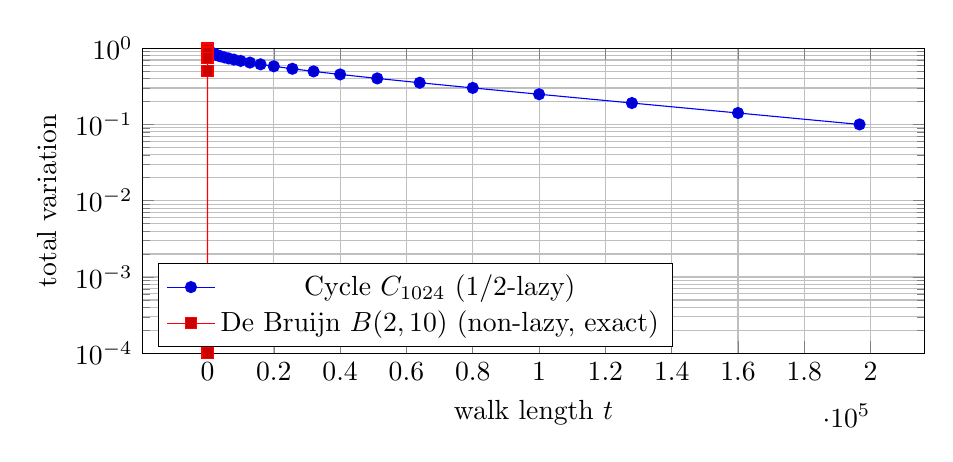
\begin{tikzpicture}
\begin{axis}[
  xmode=linear,
  width=0.95\linewidth,
  height=0.45\linewidth,
  xlabel={walk length $t$},
  ylabel={total variation},
  ymin=1e-4, ymax=1,
  ymode=log,
  legend style={at={(0.02,0.02)},anchor=south west},
  grid=both,
  unbounded coords=jump,
]
\addplot coordinates {
(1,0.997070)
(2,0.995117)
(3,0.993164)
(4,0.991211)
(5,0.989258)
(6,0.988770)
(8,0.986786)
(10,0.984949)
(12,0.983808)
(16,0.981296)
(20,0.979224)
(25,0.976890)
(32,0.974023)
(40,0.971308)
(50,0.968162)
(64,0.964399)
(80,0.960551)
(100,0.956326)
(128,0.951236)
(160,0.946076)
(200,0.940398)
(256,0.933467)
(320,0.926533)
(400,0.918901)
(512,0.909569)
(640,0.900256)
(800,0.890021)
(1000,0.878799)
(1280,0.865131)
(1600,0.851514)
(2000,0.836606)
(2560,0.818464)
(3200,0.800483)
(4000,0.780843)
(5120,0.757061)
(6400,0.733548)
(8000,0.707987)
(10000,0.680260)
(12800,0.646896)
(16000,0.614175)
(20000,0.578919)
(25600,0.536849)
(32000,0.495993)
(40000,0.452439)
(51200,0.401188)
(64000,0.352255)
(80000,0.301203)
(100000,0.248766)
(128000,0.190896)
(160000,0.141210)
(196657,0.100000)
};
\addlegendentry{Cycle $C_{1024}$ (1/2-lazy)}
\addplot coordinates {
(1,0.998047)
(2,0.996094)
(3,0.992188)
(4,0.984375)
(5,0.968750)
(6,0.937500)
(7,0.875000)
(8,0.750000)
(9,0.500000)
(10,1e-4)
(11,1e-4)
(12,1e-4)
};
\addlegendentry{De Bruijn $B(2,10)$ (non-lazy, exact)}
\end{axis}
\end{tikzpicture}
\caption{Smooth decay vs.\ finite-time cutoff in $\TV$. For log-$y$ display, exact zeros are clipped to $10^{-4}$.}
\label{fig:tv-cliff}
\end{figure}

\paragraph{Scaling check for the Chord ring+fingers overlay.}
Because the ring+fingers kernel is a circulant (Cayley) digraph on $\mathbb{Z}_n$,
the distribution and $\sigma=\max_{k\neq 0}|\lambda_k|$ can be computed exactly
by FFT. \cref{tab:chord-scale} reports $t_{0.1}$ and separation as $n=2^m$ grows.

\begin{table}[h]
\centering
\small
\setlength{\tabcolsep}{4pt}
\begin{tabular}{rrrrrrr}
\toprule
$n$ & $m$ & $\sigma$ & measured $t_{0.1}$ & TV@ $t_{0.1}$ & Sep@ $t_{0.1}$ & pred.\ $t_{0.1}$ \\
\midrule
256 & 8 & 0.875000 & 14 & 0.0963 & 0.7028 & 33 \\
512 & 9 & 0.888889 & 16 & 0.0978 & 0.7346 & 41 \\
1024 & 10 & 0.900000 & 18 & 0.0989 & 0.7633 & 49 \\
2048 & 11 & 0.909091 & 21 & 0.0876 & 0.7270 & 57 \\
\bottomrule
\end{tabular}
\caption{Chord ring+fingers scaling (1/2-lazy, start 0).}
\label{tab:chord-scale}
\end{table}



\paragraph{Sensitivity to compromise fraction: time-hidden first-hit.}
We sweep compromised fraction $\alpha$ and report (i) the probability of hitting
the compromised set within a horizon of 30 steps and (ii) leakage in a
\emph{time-hidden} model where the adversary learns only which compromised node
was hit first. (Construction details are in \cref{sec:reconstruct}.)

\begin{table}[h]
\centering
\small
\setlength{\tabcolsep}{3.5pt}
\begin{tabular}{r|rrr|rrr}
\toprule
 & \multicolumn{3}{c|}{Chord ring+fingers} & \multicolumn{3}{c}{Random 8-regular} \\
comp.\ frac & $P[\mathrm{hit}\le 30]$ & $I_{\mathrm{hid}}$ (bits) & MAP$_{\mathrm{hid}}$ &
$P[\mathrm{hit}\le 30]$ & $I_{\mathrm{hid}}$ (bits) & MAP$_{\mathrm{hid}}$ \\
\midrule
0.01 & 0.135986 & 0.046782 & 0.002159 & 0.118898 & 0.041077 & 0.002449 \\
0.05 & 0.526431 & 0.263719 & 0.007143 & 0.486559 & 0.237269 & 0.008565 \\
0.10 & 0.779561 & 0.587120 & 0.013865 & 0.742507 & 0.534519 & 0.017125 \\
0.20 & 0.958342 & 1.365357 & 0.029827 & 0.930654 & 1.236780 & 0.036783 \\
\bottomrule
\end{tabular}
\caption{Sanity-check ``first-hit'' sensitivity to compromised fraction ($n=1024$, horizon 30).}
\label{tab:firsthit-sweep}
\end{table}

\section{Reconstruction specification (compact)}\label{sec:reconstruct}
This section specifies enough to reconstruct \cref{tab:families,tab:firsthit-sweep}
from scratch. The goal is \emph{interoperable reimplementation}: an independent
implementation (human or LLM-generated) should reproduce values up to small
numerical tolerance.

\subsection{Graph families and kernels}
All kernels use \textbf{1/2-laziness}: with probability $1/2$ stay put; with
probability $1/2$ take a uniform random outgoing step.
All graphs are on $V=\{0,1,\dots,n-1\}$ with $n=1024$ unless stated.

\begin{itemize}[leftmargin=1.2em]
\item \textbf{Cycle $C_n$.} Undirected edges $(i,i\pm1\bmod n)$. Lazy walk as above.
\item \textbf{2D torus.} Grid $(\mathbb{Z}/32\mathbb{Z})^2$ mapped to $0..1023$;
neighbors differ by $\pm1$ in one coordinate (4-neighborhood); lazy walk.
\item \textbf{Hypercube $Q_{10}$.} Nodes are 10-bit strings; neighbors differ in
one bit (degree 10); lazy walk.
\item \textbf{Random 8-regular.} Sample an undirected 8-regular graph uniformly
at random (e.g., \texttt{networkx.random\_regular\_graph}) with RNG seed 0; lazy walk.
\item \textbf{Chord ring+fingers (directed).} Let $n=2^{10}$. From node $x$,
out-neighbors are $x+2^j\bmod n$ for $j=0,\dots,9$ (outdegree 10). Use the lazy
out-neighbor walk. (This digraph is regular and Eulerian, so $\pi$ is uniform.)
\item \textbf{Directed de Bruijn $B(2,10)$.} Nodes are length-10 bitstrings.
A move shifts left and appends a fresh random bit; use 1/2-laziness. (Uniform $\pi$.)
\end{itemize}

\subsection{Metrics and procedures}
\paragraph{Stationary distribution.}
For the regular families above, $\pi=\Unif(V)$. If implementing variants that
are not Eulerian, compute $\pi$ by power iteration until $\|\pi P-\pi\|_\infty$
is below $10^{-12}$.

\paragraph{TV and separation.}
Starting from the point mass at node 0, iterate $p_{t+1}=p_t P$.
Compute $\TV(p_t,\pi)=\tfrac12\sum_x|p_t(x)-\pi(x)|$ and
$\mathrm{sep}(p_t,\pi)=1-\min_x p_t(x)/\pi(x)$.

\paragraph{$t_{0.1}$.}
Define $t_{0.1}=\min\{t:\TV(p_t,\pi)\le 0.1\}$.

\paragraph{Singular value $\sigma$.}
Compute $\sigma=\sigma_2(\cD)$ where $\cD=\Pi^{1/2}P\Pi^{-1/2}$.
For uniform $\pi$, $\cD=P$. In sparse form, estimate the top singular values via
Lanczos/ARPACK SVD; report $\sigma_2$ to 6 decimals.

\paragraph{Predicted $t_{0.1}$.}
Solve for the smallest integer $t$ such that
$\tfrac12\sqrt{n}\,\sigma^{t}\le 0.1$ (using $\|v\|_1\le\sqrt{n}\|v\|_2$).

\subsection{First-hit time-hidden compromise sweep}
Fix horizon $H=30$ and compromised fraction $\alpha\in\{0.01,0.05,0.10,0.20\}$.
For each $\alpha$, sample a compromised set $C$ of size $\lfloor \alpha n\rfloor$
uniformly at random (seed 0). Sample $S\sim\Unif(V)$ and run a length-$H$ lazy
walk from $S$. Let $Y$ be the identity of the \emph{first} node in $C$ hit
(if any), else a special symbol $\bot$. In the \emph{time-hidden} model the
adversary observes $Y$.

Estimate:
\[
I_{\mathrm{hid}} = I(S;Y), \qquad
\mathrm{MAP}_{\mathrm{hid}} = \Prb[\hat S(Y)=S]\ \text{for the Bayes-optimal }\hat S.
\]
Use Monte Carlo with at least $10^5$ trials per $\alpha$; the shipped JSON records fixed raw anchors rather than long Monte Carlo logs.
Treat results within $\pm 0.02$ bits (MI) and $\pm 2\times10^{-3}$ (MAP) as matching.

\paragraph{Sanity anchors.}
An implementation consistent with the above should reproduce
\cref{tab:families,tab:firsthit-sweep} within the stated tolerances.

\section{Conclusion}
Time reversal makes random-walk delegation anonymity explicit: the observed
delegate reveals a reversed walk. This yields sharp optimal distinguishability
and computable leakage certificates for directed overlays, and clarifies why
single-parameter spectral heuristics can fail on non-normal kernels. We provide
compact reconstruction guidance here to enable straightforward reimplementation.


\paragraph{Artifact availability.}
The source-only supplement shipped with this archive,
\texttt{published/2026-01-23\_spectral\_anonymity/supplement/}, contains
\texttt{spectral\_reconstruction.py} and
\texttt{spectral\_sanity\_outputs.json}.  It records the raw anchors for the
tables and figure coordinates and gives executable helpers for the exact
$t$-step Frobenius witness, the conservative $\sigma_2$ certificate, the
normality-gated shortcut, common-stationary inhomogeneous-product sanity checks,
observation-channel, joint-observation composition, adaptive-transcript composition, post-processing/coarsening, tail-under-coarsening, hidden-selector, adaptive-selector, prior-baseline-minimum, estimator-certification, estimator-confidence/multiplicity accounting, kernel/model uncertainty, numeric/serialization precision, separation-vs-upper-ratio, pairwise/session support, and visible-vs-hidden-hopcount sanity checks, arbitrary-prior
and stop-time-visibility sanity checks, expected-to-tail / exact weighted-quantile
$\chi^2$ translation helpers, plus compact raw/archive guard
checks (including \texttt{--joint-observation-sanity}, \texttt{--adaptive-transcript-sanity}, \texttt{--estimator-certification-sanity}, \texttt{--estimator-multiplicity-sanity}, \texttt{--numeric-serialization-sanity}, \texttt{--check-raw}, and \texttt{--archive-guard}). Rendered plots and long
logs remain transient rather than shipped archive files.


\section*{References}
\begin{thebibliography}{99}\small

\bibitem{lpw}
D.~A. Levin, Y.~Peres, and E.~L. Wilmer.
\newblock \emph{Markov Chains and Mixing Times}, 2nd ed.
\newblock American Mathematical Society, 2017.

\bibitem{aldousdiaconis}
D.~Aldous and P.~Diaconis.
\newblock Strong stationary times and finite random walks.
\newblock \emph{Advances in Applied Mathematics}, 2(1):69--97, 1987.

\bibitem{fill}
J.~A. Fill.
\newblock The strength of weak convergence.
\newblock \emph{Stochastic Processes and their Applications}, 87(1):1--10, 2000.

\bibitem{reiterrubin}
M.~K. Reiter and A.~D. Rubin.
\newblock Crowds: Anonymity for {W}eb transactions.
\newblock \emph{ACM Transactions on Information and System Security}, 1(1):66--92, 1998.

\bibitem{backes}
M.~Backes, I.~Goldberg, A.~Kate, and T.~Toft.
\newblock Adding query privacy to robust {DHT}s.
\newblock In \emph{Proceedings of ASIACCS}, 2012.



\bibitem{shadowwalker}
P.~Mittal and N.~Borisov.
\newblock ShadowWalker: Peer-to-peer anonymous communication using redundant structured topologies.
\newblock In \emph{Proceedings of the 16th ACM Conference on Computer and Communications Security (CCS)}, 2009.

\bibitem{nisan}
A.~Panchenko, S.~Richter, and A.~Rache.
\newblock NISAN: Network information service for anonymization networks.
\newblock In \emph{Proceedings of the 16th ACM Conference on Computer and Communications Security (CCS)}, pages 141--150, 2009.

\bibitem{octopus}
Q.~Wang and N.~Borisov.
\newblock Octopus: A secure and anonymous DHT lookup.
\newblock In \emph{Proceedings of the 32nd IEEE International Conference on Distributed Computing Systems (ICDCS)}, pages 325--334, 2012.
\end{thebibliography}

\end{document}
